
%(BEGIN_QUESTION)
% Copyright 2010, Tony R. Kuphaldt, released under the Creative Commons Attribution License (v 1.0)
% This means you may do almost anything with this work of mine, so long as you give me proper credit

An industrial furnace fueled by wood waste (sawdust, splintered boards, scraps) uses a conveyor belt to move fuel into the furnace.  The belt is is moved by an AC motor powered through a variable frequency drive (VFD), so that the feed rate may be adjusted automatically by a PLC.  The PLC's tasks is to monitor furnace temperature by the average measurement of multiple temperature sensors and maintain this average by adjusting the conveyor speed accordingly:

$$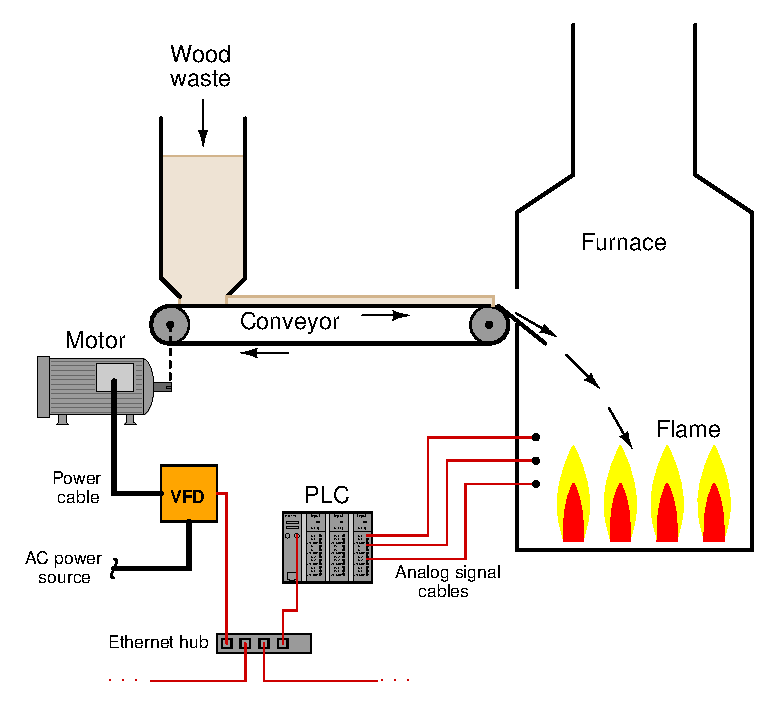
\includegraphics[width=15.5cm]{i04566x01.eps}$$

Digital signals sent to the VFD through Ethernet cables give it speed commands, with the PLC sending a new speed command to the drive only when the speed needs to change (i.e. it doesn't just keep sending the same speed command if that speed is correct).

\vskip 10pt

One day someone's office computer at the facility plugged into the same hub fails in such a way that it begins to constantly ``jabber.''  Answer the following questions:

\vskip 10pt

\begin{itemize}
\item{} What effect might this fault have on the furnace's actual temperature?
\vskip 10pt
\item{} What diagnostic indications might a technician look for to identify the nature of the problem?
\vskip 10pt
\item{} How could this type of problem be avoided in the future?
\end{itemize}

\underbar{file i04566}
%(END_QUESTION)





%(BEGIN_ANSWER)

I recommend 4 points for the diagnostic answer, and 3 points each for the others:

\begin{itemize}
\item{} What effect might this fault have on the furnace's actual temperature? {\bf The temperature may drift off setpoint (either high or low, depending on furnace conditions and the last speed command received by the VFD.  It is possible the temperature may hold steady, if fuel supply feed rate just happens to meet demand.}
\vskip 10pt
\item{} What diagnostic indications might a technician look for to identify the nature of the problem? {\bf LEDs on the hub may indicate traffic at the offending port, the inability to ``ping'' devices on this collision domain would be another test.}
\vskip 10pt
\item{} How could this type of problem be avoided in the future? {\bf Use a dedicated hub for the process control system (not one shared by cheap office computers), install Ethernet interfaces with ``jabber latch'' features, or simply go with analog signaling between the PLC and the VFD.}
\end{itemize}

Half-credit (2 points) should be awarded to diagnostic tests that don't specifically reveal this to be a network problem.

%(END_ANSWER)





%(BEGIN_NOTES)

{\bf This question is intended for exams only and not worksheets!}.

%(END_NOTES)

